\documentclass[xcolor=dvipsnames,14pt,professionalfonts]{beamer}
\usepackage{minted}
\usepackage{etoolbox}
\usepackage[T1]{fontenc}
\usepackage{lmodern}
\usepackage[no-math]{fontspec} 
\usetheme{rsmarttraining}
\usefonttheme{professionalfonts}
\usecolortheme{dolphin}

%\definecolor{foreground}{gray}{0}
%\definecolor{background}{gray}{1}
%\definecolor{keyword}{rgb}{0.2,0.2,0.8}
%\definecolor{warning}{rgb}{0.8,0.2,0.2}
%\definecolor{shadow}{gray}{0.35}
%\definecolor{hide}{gray}{0.9}
%\definecolor{figure}{rgb}{1,0.7,0}
%\definecolor{title}{rgb}{25,240,250}
\definecolor{title}{rgb}{0.09,0.30,0.38}
\definecolor{frametitle}{rgb}{1,1,1}
\definecolor{normal}{rgb}{0,0,0}

%\usecolortheme[named=keyword]{structure}

\setbeamercolor{title}{fg=title}
\setbeamercolor{frametitle}{fg=frametitle}
\setbeamercolor{section in toc}{fg=foreground}
\setbeamercolor{normal text}{bg=brown!46,fg=normal}

\setbeamerfont{structure}{family=\fontspec{Georgia},series=\bfseries} 
\setbeamerfont{subtitle}{family=\fontspec{Helvetica},series=\bfseries} 
\begin{document}

\title{KRAD Training}
\subtitle{Exercise: Maintenance Documents Part 1}
\author[Leo]{Leo Przybylski}

\usebackgroundtemplate%
{%
    
\includegraphics[width=\paperwidth,height=\paperheight]{../img/header.png}%
}

{
\usebackgroundtemplate{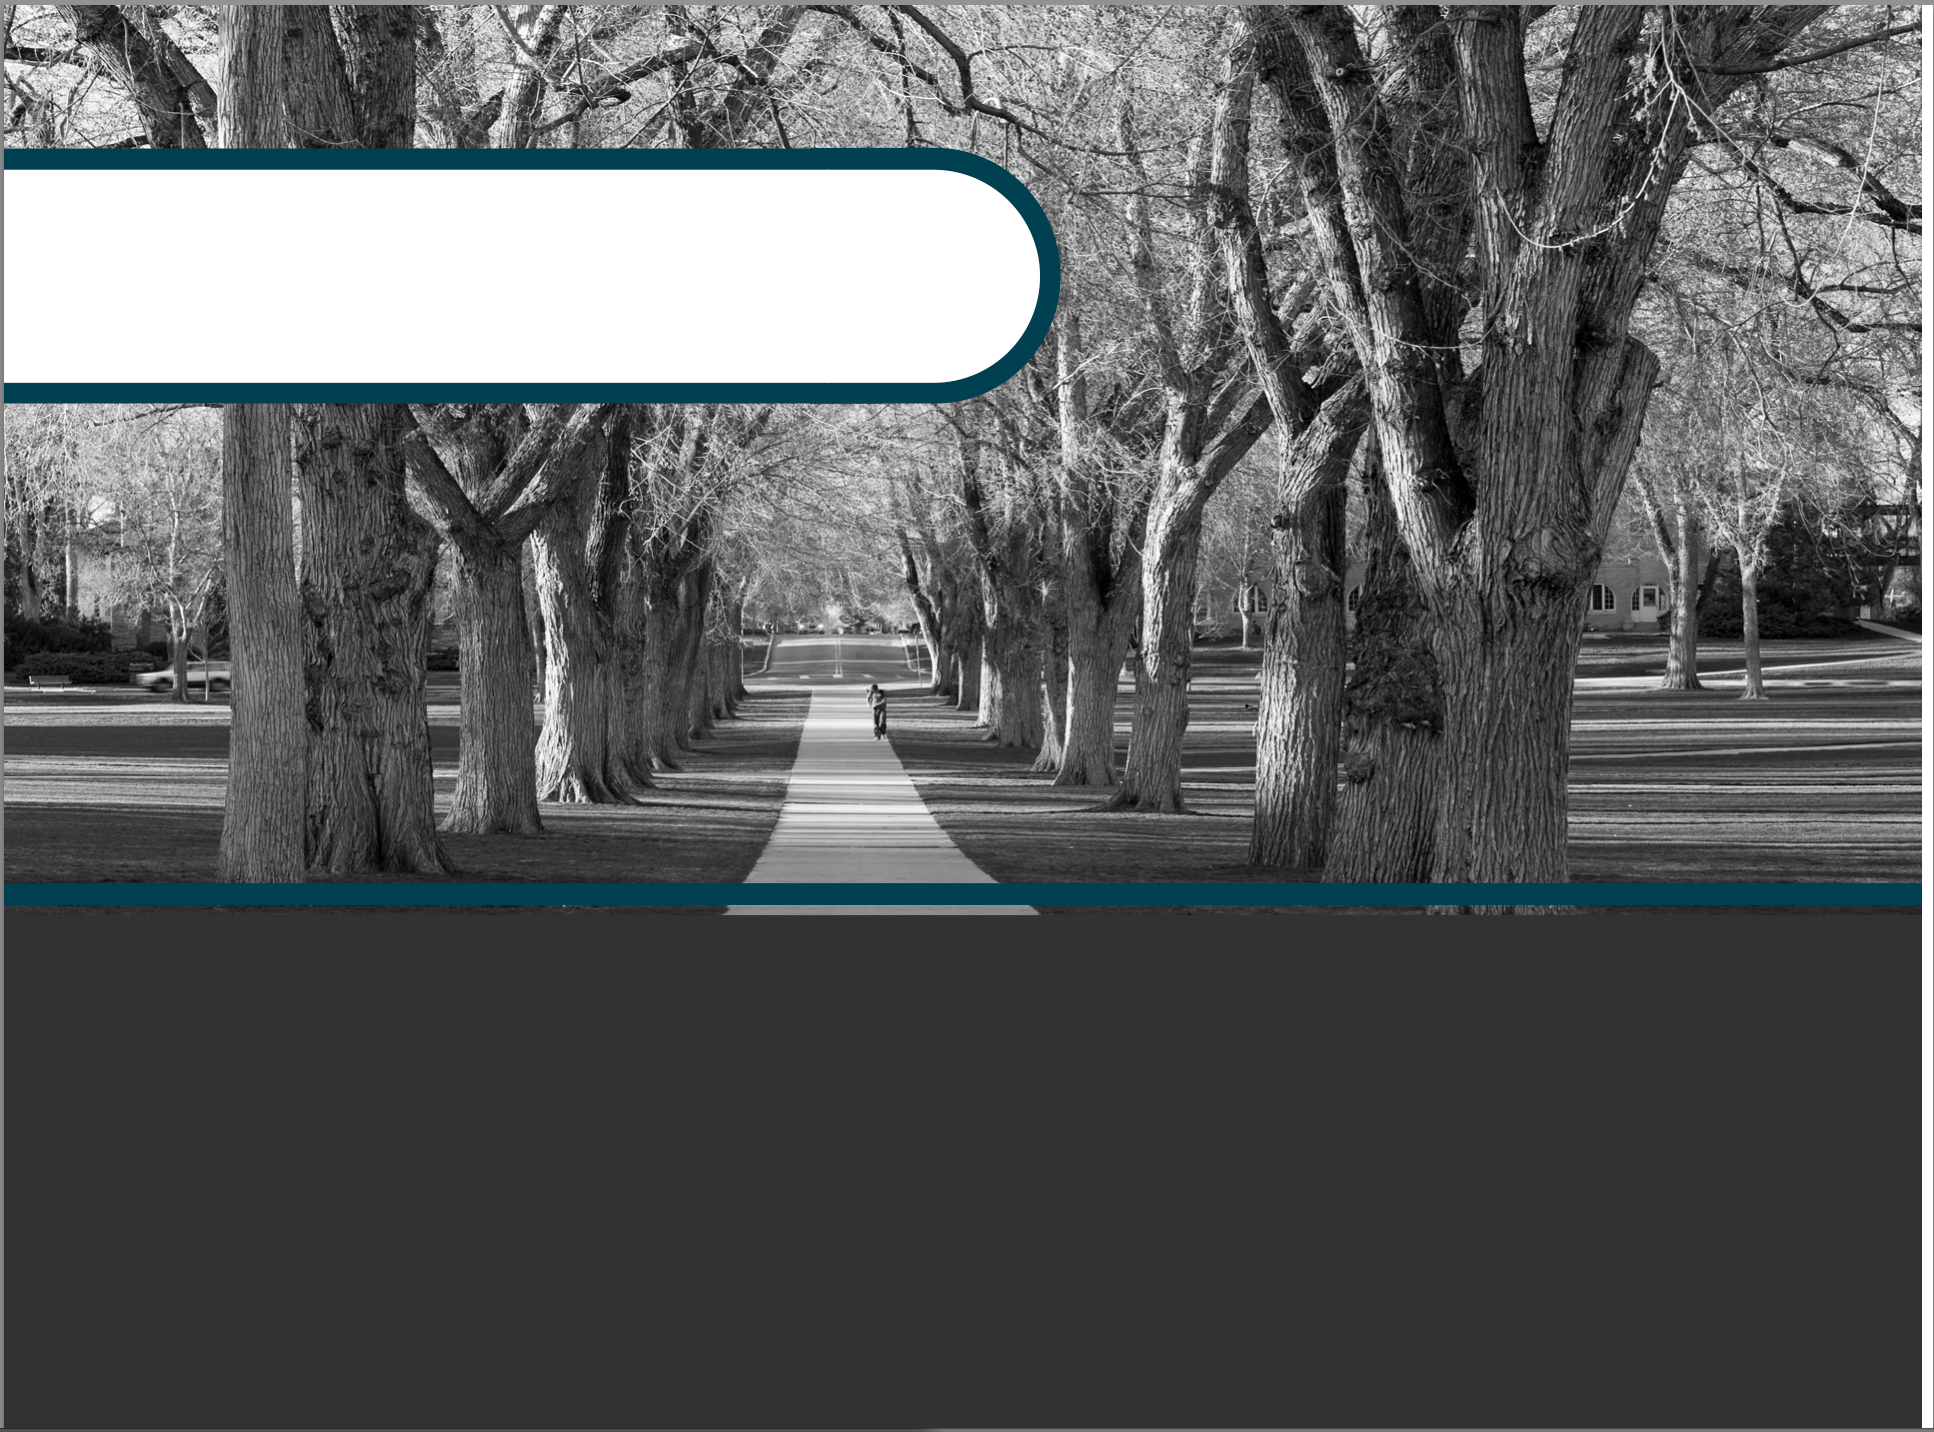
\includegraphics[width=\paperwidth]{../img/title.png}}%
\begin{frame}[plain]
  \titlepage
\end{frame}
}

\begin{frame}{Goals}
  \begin{itemize}
    \item Create a Maintenance Document for maintaining Authors.
    \item Create a Maintenance Document for maintaining Books.
  \end{itemize}
\end{frame}
\begin{frame}{Checkout exercise-krad-maint-doc project}
  To ensure a clean and consistent environment for everyone, we will check out a project from Subversion as a starting point.  This will essentially be a completed copy of the previous exercises.
In order to get the copy of the project that you will need, please
check out the exercise-maint-doc project from the training Subversion
repository.
\end{frame}
\begin{frame}{Create Author Maintenance Document}
  In this part of the exercise, we will create a simple document
    for Author maintenance.  There will be no workflow or routing
    associated with this document (we’ll get to that later!).
\end{frame}

\begin{frame}{Create Author Maintenance Document}
  We have already created a few pieces to get you started, read below for instructions:
  \begin{enumerate}
  \item Open the \texttt{AuthorMaintenanceDocument.xml} file located in the project at \texttt{src/main/resources/trnapp/bookstore/}.
  \item Read through what is currently in this file and take some time to try and understand it.
  \item Notice that we’ve already created the
    uifMaintenanceDocumentEntry and \texttt{Uif-MaintenanceView} for you.  This is a maintenance document with a single section that contains the lastName.
  \end{enumerate}
\end{frame}

\begin{frame}{Create Author Maintenance Document}
  \begin{enumerate}
  \item Add \texttt{Uif-InputField} elements for firstName and middleName.
  \item Make firstName textbf{required}.
  \item We have already added this data dictionary file for you to the list in \texttt{Module.xml}.
  \item Finally, in order to create new instances of the maintenance document, we need to set up a workflow Document Type.
  \end{enumerate}
\end{frame}

\begin{frame}{Create Author Maintenance Document}
  \begin{enumerate}
  \item Notice the documentTypeName on the maintenance entry is set to \textbf{AuthorDocumentType}.
  \item This means that Kuali Enterprise Workflow needs to have \textbf{AuthorDocumentType} configured in order for this maintenance document to be functional.
  \item This means that Kuali Enterprise Workflow needs to have \textbf{AuthorDocumentType} configured in order for this maintenance document to be functional.
  \end{enumerate}
\end{frame}

\begin{frame}{Create Author Maintenance Document}
  \begin{enumerate}
  \item We have created a simple workflow document type definition for \textbf{AuthorDocumentType} which can be found under \texttt{workflow/AuthorDocumentType.xml}.
  \item This document type currently defines no workflow route path.
    It also uses RiceDocument as its parent to allow us to inherit
    Kuali Identity Management permissions from the parent (as well as
    other things).  We’ll get to both of those pieces in more detail in a later exercise.
  \end{enumerate}
\end{frame}

\begin{frame}{Create Author Maintenance Document}
  \begin{enumerate}
  \item Next, we need to “ingest” this document type into Kuali Enterprise Workflow.  This installs the document type and its associated workflow process definition into the Rice database.  Start the web application and navigate to the main portal page.
  \item Once on the main portal page, click on the “Administration”
    tab and log in as “admin”.
  \end{enumerate}
\end{frame}

\begin{frame}{Create Author Maintenance Document}
  In the “Workflow” sub-menu, click on “XML Ingester” .
  \begin{enumerate}
  \item On the resulting screen, browse for AuthorDocumentType.xml and click the “upload xml data” button.  If it succeeds, you should see the following:
  \end{enumerate}
\end{frame}

\begin{frame}{Test the Author Maintenance Document}
  You should now be able to test your changes to the Author maintenance document.
  \begin{enumerate}
    \item Launch the web application and navigate to the Author lookup
    \item Notice that a “Create New” button now appears in the top right corner of the Author lookup:
    \item Click the “Create New” button.  This will launch your maintenance document.  It should look something like the following:
  \end{enumerate}
\end{frame}

\begin{frame}{Test the Author Maintenance Document}
  \begin{enumerate}
  \item Fill out the form to create a new Author and hit the “submit” button.
  \item Navigate back to the Author lookup and do a search to verify that your new Author was successfully entered into the database.
  \item Next, try to edit the Author that you just created.
  \item To do this, execute a search on the Author lookup screen.
  \item You should now see an “edit” and a “copy” button next to each row in the result set.  Click “edit” on the Author you just created.
  \end{enumerate}
\end{frame}

\begin{frame}{Test the Author Maintenance Document}
  \begin{enumerate}
  \item Notice how the resulting maintenance screen brings up a side-by-side view of the original Author attributes and allows you to change them on the right-hand side:
  \item Try making a change (such as modifying one of the names, or adding a middle name).
  \item Submit the maintenance document.
  \item Navigate back to your Author lookup and execute another search.  You should see the updates to the Author that you changed now.
  \end{enumerate}
\end{frame}

\begin{frame}{Test the Author Maintenance Document}
  \begin{enumerate}
  \item Find your Author Maintenance Transactions in Document Search
  \item We mentioned previously that you were not going to be configuring any Workflow for this part of the exercise.  However, the submission of the various Author maintenance documents that you have already done have been routing through Kuali Enterprise Workflow.
    \item The AuthorDocumentType has not been set up with any routing nodes or routing rules, so the document never stops during the routing process.  This is the reason why the change appears to happen (almost) instantly to us.
  \end{enumerate}
\end{frame}

\begin{frame}{Test the Author Maintenance Document}
  \begin{enumerate}
  \item To see the workflow documents that have been created during your testing, follow these steps:
  \item Navigate to the “Main Menu” in your portal.
  \item Click on the “doc search” button near the top.
  \item On the resulting screen, click the “search” button.  This will search for all documents created today.
  \item You should see results similar to the following:
  \end{enumerate}
\end{frame}

 \begin{frame}{Create Book Maintenance Document}
In this part of the exercise, you will implement the maintenance document for Book yourself.
There are a few steps that you will need to follow here: 
 \begin{enumerate}
 \item Create a BookDocumentType.xml file to define your workflow document type and use the “XML Ingester” screen to ingest it.  Use AuthorDocumentType.xml as an example to start from.
 \item Create a BookMaintenanceDocument.xml file which contains the data dictionary configuration for your Book maintenance document.  When creating this, please do the following:
   \item As with the Inquiry you created earlier, create a main “Book Maintenance” section and a “Publishing Information” section.
  \end{enumerate}
\end{frame}
 
\begin{frame}{Create Book Maintenance Document}
  \begin{enumerate}
    \item In the “Book Maintenance” section, put the following fields:
      \begin{itemize}
      \item title
      \item authorId
      \item isbn
      \item category
\end{itemize}
  \end{enumerate}
\end{frame}

\begin{frame}{Create Book Maintenance Document}
  \begin{enumerate}
  \item In the “Publishing Information” section, put the following fields:
      \begin{itemize}
      \item publisher
      \item publicationDate
\end{itemize}
\item Add a reference to your \texttt{BookMaintenanceDocument.xml} data
  dictionary file in \texttt{Module.xml} so that it will get loaded on startup.
  \end{enumerate}
\end{frame}
 
\begin{frame}{Test the Book Maintenance Document}
  \begin{enumerate}
  \item You should now be able to test your Book maintenance document.
  \item Launch your web application and navigate to the Book lookup screen.
  \item You should see a \textbf{Create New} button link here as well.
  \item If you don’t see this link, be sure you added your new data dictionary file in Module.xml
  \item If that checks out, double-check that you ingested the new BookDocumentType using the “XML Ingester” screen
    \end{enumerate}
  \end{frame}

\begin{frame}{Test the Book Maintenance Document}
   When you create a new Book, you should see a screen like the
    following:
    Try creating a few Books in order to test that your maintenance document is working properly.
  \end{frame}
\end{document}
